% !TeX root = Protokoll.tex
\subsection{Drehschieberpumpe}
In den Folgenden Abschnitten werden die, unter Verwendung der Drehschieberpumpe, aufgenommenen Messreihen 
zur Evakuierungskurve und der Leckratenmessung ausgewertet. Mit den Ergebnissen aus diesen, folgt im letzten Teil dieses 
Abschnitts die Betrachtung des Saugvermögens in Abhängigkeit des Druckes.

\subsubsection{Evakuierungskurve}
Die zur Bestimmung der Evakuierungskurve aufgenommenen Messwerte für den Druck
im Rezipienten sind in \cref{tab:Evakuierungskurve_Drehschieber} auch als logarithmierte
Werte zu finden. Für die Logarithmierung wurden der Maximaldruck $p_{0} =\SI{100(30)}{\milli\bar} $
und der in dieser Messreihe festgestellte Enddruck $p_{\mathrm{e}} =\SI{20(6)}{\micro\bar}$ verwendet.
Der Messfehler der Druckwerte wurde aufgrund der Herstellerangabe \cite{Pfeifer} mit \SI{30}{\percent} angenommen.
Neben den Messwerten für den Druck sind auch die, über die fünf Messungen, gemittelten Messwerte der Zeit 
angegeben. Der Messfehler der Zeit ist dabei für jeder der fünf Messungen mit $\sigma_{t} = \SI{1}{\s}$ als systematischer
Fehler angenommen, sodass sich dieser durch die Mittlung nicht verringert.

%Tabelle der Messwerte
\begin{table}[!h]
	\centering
	\begin{tabular}{cccccc}
		\toprule
		Druck & logarithm. Druck & gemittelte Zeit & Druck & logarithm. Druck & gemittelte Zeit\\
		$p$/\si{mbar} & $\frac{p-p_e}{p_0-p_e}$ & $\bar{t}$/\si{s} & $p$/\si{mbar} & $\frac{p-p_e}{p_0-p_e}$ & $\bar{t}$/\si{s}\\
\midrule
		\num{100(30)} & \num{0.0(0)} & \num{14(1)} & \num{1.0(3)} & \num{-4.6(4)} & \num{73(1)}\\
		\num{60(18)} & \num{-0.5(4)} & \num{25(1)} & \num{0.8(2)} & \num{-4.9(4)} & \num{75(1)}\\
		\num{40(12)} & \num{-0.9(4)} & \num{32(1)} & \num{0.6(2)} & \num{-5.1(4)} & \num{80(1)}\\
		\num{20(6)} & \num{-1.6(4)} & \num{41(1)} & \num{0.4(1)} & \num{-5.6(4)} & \num{88(1)}\\
		\num{10(3)} & \num{-2.3(4)} & \num{49(1)} & \num{0.20(6)} & \num{-6.3(4)} & \num{104(1)}\\
		\num{8(2)} & \num{-2.5(4)} & \num{51(1)} & \num{0.10(3)} & \num{-7.1(5)} & \num{121(1)}\\
		\num{6(2)} & \num{-2.8(4)} & \num{54(1)} & \num{0.08(2)} & \num{-7.4(5)} & \num{130(1)}\\
		\num{4(1)} & \num{-3.2(4)} & \num{58(1)} & \num{0.06(2)} & \num{-7.8(6)} & \num{149(1)}\\
		\num{2.0(6)} & \num{-3.9(4)} & \num{65(1)} & \num{0.04(1)} & \num{-8.5(7)} & \num{214(1)}\\
		\bottomrule
	\end{tabular}
	\caption{Werte der Messung der Evakuierungskurve unter Verwendung der Drehschieberpumpe.
                        Neben den gemessenen Drücken sind auch die logarithmierten Drücke und die gemittelten
                        Zeiten angegeben. Dabei sind die Fehler der Zeiten systematischen Ursprungs und wurden 
                        daher durch das Mitteln nicht reduziert. \label{tab:Evakuierungskurve_Drehschieber}}
\end{table}


In \cref{fig:evakuierungskurve_drehschieber_exp} sind die Messwerte für den Druck gegen die der Zeit aufgetragen,
sodass ich ein exponentieller Verlauf der Evakuierungskurve zeigt. Da ein solcher Verlauf, wie in 
\eqref{eq:Evakuierungskurve} hergeleitet, jedoch nur für ein konstantes Saugvermögen gilt, werden für dessen Bestimmung die logarithmierten Werte der Drücke gegen die Zeit aufgetragen.
In dieser Darstellung lassen sich drei Druckbereiche ausmachen,
in denen die Messwerte einen linearen Verlauf zeigen. Die grafische Darstellung der Messwerte und die 
Ausgleichesgeraden für den jeweiligen Druckbereich sind in den Abbildungen \ref{fig:evakuierungskurve_drehschieber_log_0} 
bis \ref{fig:evakuierungskurve_drehschieber_log_2} dargestellt.\\



{%Exponential-Darstellung der Messdaten
\begin{figure}[!h]
 \centering
 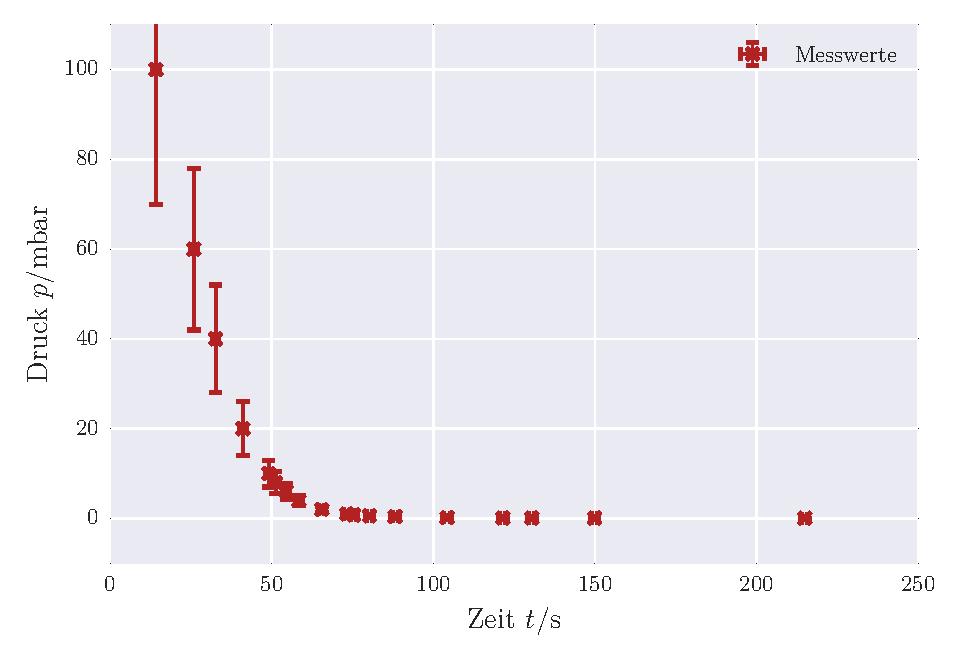
\includegraphics[scale=.9]{../Grafiken/Evakuierungskurve_Drehschieber_exp.pdf}
 \caption{Grafische Darstellung der aufgenommenen Evakuierungskurve der Drehschieberpumpe. \label{fig:evakuierungskurve_drehschieber_exp}}
 \end{figure} 
\FloatBarrier}

{%Logarithmische-Darstellung der Messdaten mit Fits
\begin{figure}[!h]
 \centering
 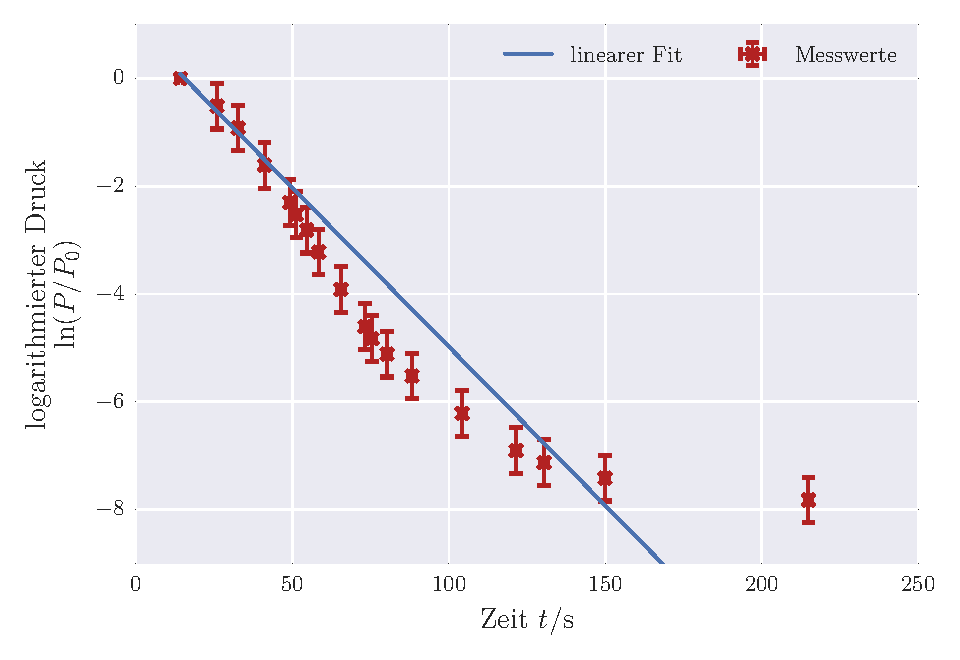
\includegraphics[scale=.80]{../Grafiken/Evakuierungskurve_Drehschieber_log_0.pdf}
 \caption{Grafische Darstellung der Evakuierungskurve mit logarithmierten Druckmesswerten und der Ausgleichsgrade für den ersten Druckbereich (\SI{100}{\milli\bar} bis \SI{20}{\milli\bar}) .\label{fig:evakuierungskurve_drehschieber_log_0}}
 \end{figure} 
\FloatBarrier
\begin{figure}[!h]
 \centering
 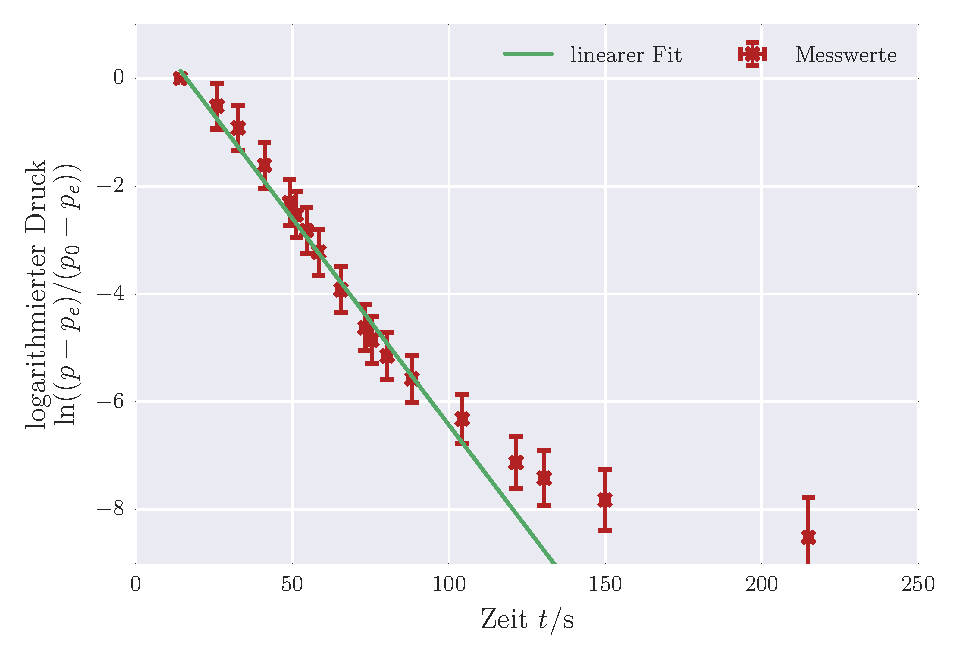
\includegraphics[scale=.80]{../Grafiken/Evakuierungskurve_Drehschieber_log_1.pdf}
 \caption{Grafische Darstellung der Evakuierungskurve mit logarithmierten Druckmesswerten und der Ausgleichsgrade für den zweiten Druckbereich (\SI{10}{\milli\bar} bis \SI{0.2}{\milli\bar}) \label{fig:evakuierungskurve_drehschieber_log_1}}
 \end{figure} 
\FloatBarrier
\begin{figure}[!h]
 \centering
 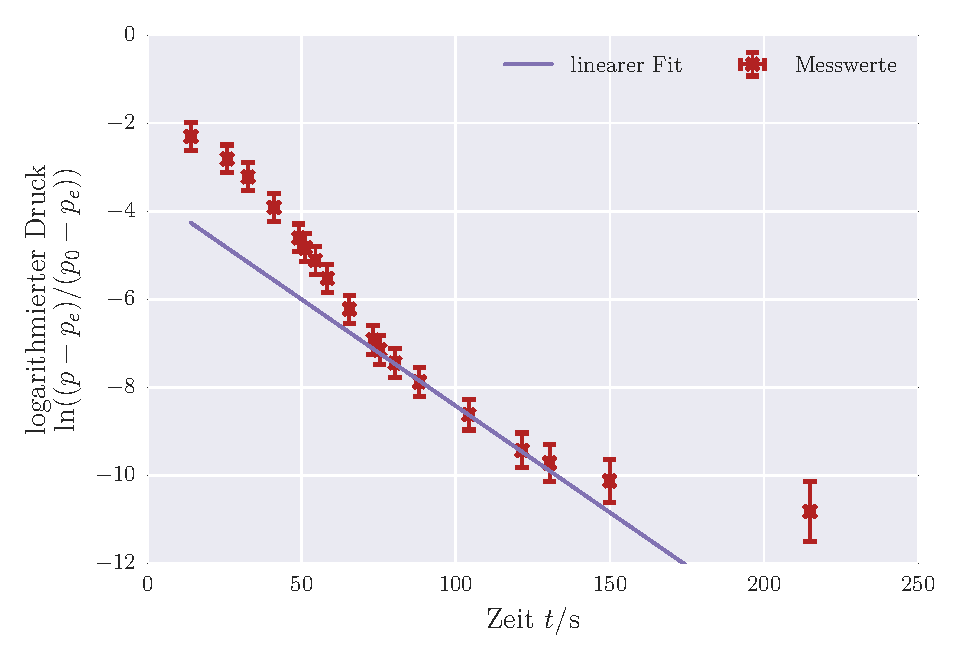
\includegraphics[scale=.80]{../Grafiken/Evakuierungskurve_Drehschieber_log_2.pdf}
 \caption{Grafische Darstellung der Evakuierungskurve mit logarithmierten Druckmesswerten und der Ausgleichsgrade für den dritten Druckbereich (\SI{0.1}{\milli\bar} bis \SI{0.04}{\milli\bar}) \label{fig:evakuierungskurve_drehschieber_log_2}}
 \end{figure} 
\FloatBarrier}

Die durchgeführte Ausgleichsrechnung für eine lineare Funktion der Form 
\begin{empheq}{equation}
P_{i}(t) = a_{i} \cdot t + b_{i}
\end{empheq}
ergab für die drei Druckbereiche $i \in [1,2,3]$ die Parameter $a_{i}$ und $b_{i}$:
{%Kopierte Fit Ergebnisse
	%Fit im 1.Bereich
	%a =  -0.0590110020632 +/- 0.0068114313639
	%b =  0.92041914012 +/- 0.20517721592
	%Fit im 2.Bereich
	%a =  -0.0766523368479 +/- 0.00477396323738
	%b =  1.23548186669 +/- 0.343789112221
	%Fit im 3.Bereich
	%a =  -0.0139336543482 +/- 0.00211667511312
	%b =  -5.57400774906 +/- 0.335411241849
}
\addtocounter{equation}{-1}
\begin{subequations}
	\begin{empheq}{align}
	a_{1} &=\SI{-0.059(7)}{\per\s}\\ 
	b_{1} &=\SI{0.9(2)}{} \notag
	\end{empheq}	                                                                                  
	\begin{empheq}{align}
	a_{2} &=\SI{-0.077(5)}{\per\s}\\ 
	b_{2} &=\SI{1.2(3)}{} \notag
	\end{empheq}
	\begin{empheq}{align}
	a_{3} &=\SI{-0.014(2)}{\per\s}\\ 
	b_{3} &=\SI{-5.6(3)}{} \notag
	\end{empheq}	
\end{subequations}\\

Aus den Steigungen $a_{i}$ der Ausgleichsgeraden lässt sich nun das Saugvermögen der Drehschieberpumpe
in dem jeweiligen Druckbereich nach \eqref{eq:Saugvermoegen_Evakuierungskurve} berechnen.
Mit dem Volumen des Rezipienten in dieser Versuchsreihe $V_{\mathrm{evak,dreh}} = \SI{10.2(7)}{\l}$ ergibt sich 
damit für das Saugvermögen:
{%Kopierte Ergebnisse
%S0 =  0.600429548171 +/- 0.0792494597197
%S1 =  0.779927918028 +/- 0.0696560633085
%S2 =  0.141773186222 +/- 0.0233708675414
}

\begin{subequations}
	\begin{empheq}{align}
	S_{1} &=\SI{0.60(8)}{\l\per\s}\\ 
	S_{2} &=\SI{0.78(7)}{\l\per\s}\\ 
	S_{3} &=\SI{0.14(2)}{\l\per\s}
	\end{empheq}	
\end{subequations}

\subsubsection{Leckratenmessung}

Die Messwerte die in den vier Messreihen der Leckraten Messung aufgenommen wurden,
sind in \cref{tab:Leckratenmessung_Drehschieber_0} dargestellt. Wiederum sind
für den Messfehler des Drucks die Herstellerangabe \cite{Pfeifer} von \SI{30}{\percent} verwendet worden.
Als Zeiten sind die Mittelwerte der dreifach ausgeführten Messungen zusammen mit dem systematischen Fehler
angegeben.  

%Tabelle zur Leckratenmessung
\begin{table}[!h]
	\centering
	\subfloat{
	\begin{tabular}{cccc}
		\toprule
		\multicolumn{2}{c}{1.Messreihe $P_g = \SI{0.10(3)}{\milli\bar}$} & \multicolumn{2}{c}{2.Messreihe $P_g = \SI{0.20(6)}{\milli\bar}$} \\\cmidrule(rl){1-2}\cmidrule(rl){3-4}
		Druck & gemittelte Zeit & Druck & gemittelte Zeit\\
		$p$/\si{mbar} & $\bar{t}$/\si{s} & $p$/\si{mbar} & $\bar{t}$/\si{s}\\
\midrule
		\num{0.20(6)} & \num{12(1)} & \num{0.4(1)} & \num{17(1)}\\
		\num{0.4(1)} & \num{64(1)} & \num{0.6(2)} & \num{46(1)}\\
		\num{0.6(2)} & \num{128(1)} & \num{0.8(2)} & \num{72(1)}\\
		\bottomrule
%	\end{tabular}
%	}\\
%	\subfloat{
%	\begin{tabular}{cccc}
		\toprule
		\multicolumn{2}{c}{3.Messreihe $P_g = \SI{0.4(1)}{\milli\bar}$ } & \multicolumn{2}{c}{4.Messreihe $P_g = \SI{0.8(2)}{\milli\bar}$} \\\cmidrule(rl){1-2}\cmidrule(rl){3-4}
		Druck & gemittelte Zeit & Druck & gemittelte Zeit\\
		$p$/\si{mbar} & $\bar{t}$/\si{s} & $p$/\si{mbar} & $\bar{t}$/\si{s}\\
		\midrule
		\num{0.6(2)} & \num{9(1)} & \num{2.0(6)} & \num{12(1)}\\
		\num{0.8(2)} & \num{18(1)} & \num{4(1)} & \num{34(1)}\\
		\num{1.0(3)} & \num{42(1)} & \num{6(2)} & \num{55(1)}\\
		\bottomrule
	\end{tabular}
	}
	
	\caption{Werte der Leckratenmessung unter Verwendung der Drehschieberpumpe.
                        Neben den gemessenen Drücken sind die gemittelten Zeiten angegeben. 
                        Dabei sind die Fehler der Zeiten systematischen Ursprungs und wurden 
                        daher durch das Mitteln nicht reduziert. \label{tab:Leckratenmessung_Drehschieber_0}}
\end{table}

\FloatBarrier
Die grafische Darstellung der jeweiligen Messreihe befindet sich in den Abbildungen \ref{fig:leckrate_drehschieber_0} 
bis \ref{fig:leckrate_drehschieber_3} jeweils zusammen mit einer durch lineare Ausgleichsrechnung bestimmten Geraden. 

{%Grafiken der Leckratenmessung
\begin{figure}[!h]
 \centering
 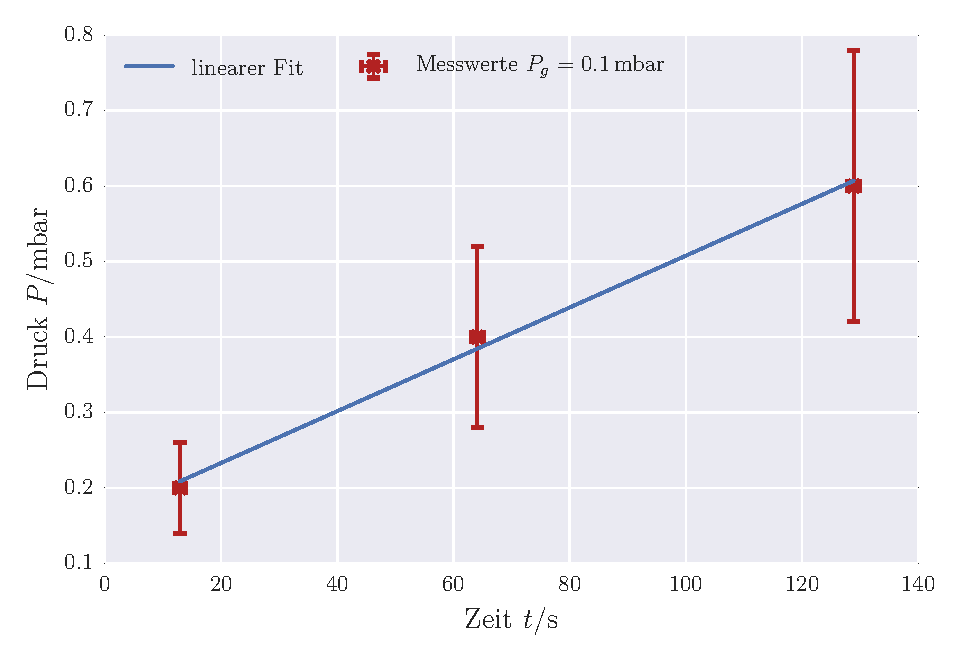
\includegraphics[scale=0.8]{../Grafiken/Leckrate_Drehschieber_0.pdf}
 \caption{Graphische Darstellung der Druckmesswerte in Abhängigkeit von der Zeit, aus der 1. Messreihe, und der
 	entsprechenden Ausgleichsgeraden. Der für die Messreihe eingestellte Gleichgewichtsdruck ist angegeben.\label{fig:leckrate_drehschieber_0}}
 \end{figure} 
\FloatBarrier
\begin{figure}[!h]
 \centering
 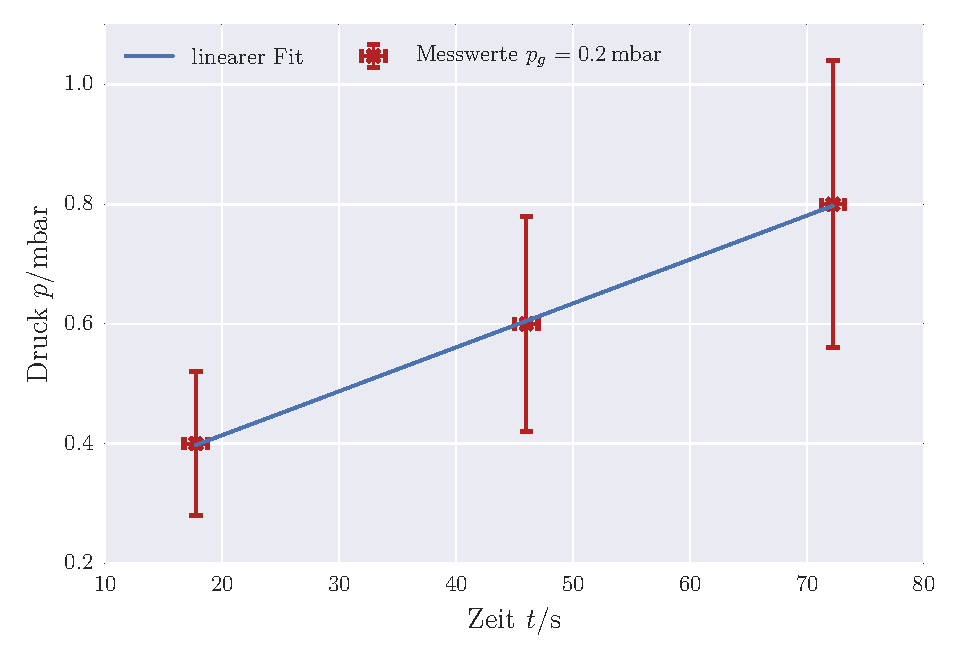
\includegraphics[scale=0.9]{../Grafiken/Leckrate_Drehschieber_1.pdf}
 \caption{Graphische Darstellung der Druckmesswerte in Abhängigkeit von der Zeit, aus der 2. Messreihe, und der
 	entsprechenden Ausgleichsgeraden. Der für die Messreihe eingestellte Gleichgewichtsdruck ist angegeben.\label{fig:leckrate_drehschieber_1}}
 \end{figure} 
\FloatBarrier
\begin{figure}[!h]
 \centering
 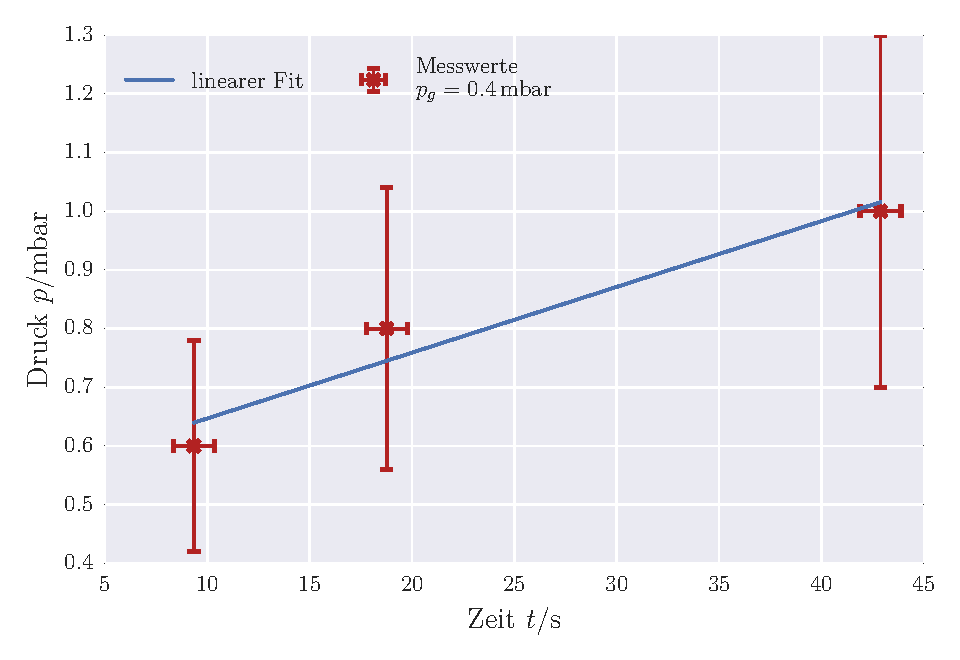
\includegraphics[scale=0.8]{../Grafiken/Leckrate_Drehschieber_2.pdf}
 \caption{Graphische Darstellung der Druckmesswerte in Abhängigkeit von der Zeit, aus der 3. Messreihe, und der
 	entsprechenden Ausgleichsgeraden. Der für die Messreihe eingestellte Gleichgewichtsdruck ist angegeben und als Messwert für $t=0$ mit eingetragen. Dieser ist grau dargestellt, da er für die 
 	Berechnung der Ausgleichsgeraden nicht verwendet wurde. \label{fig:leckrate_drehschieber_2}}
 \end{figure} 
\FloatBarrier
\begin{figure}[!h]
 \centering
 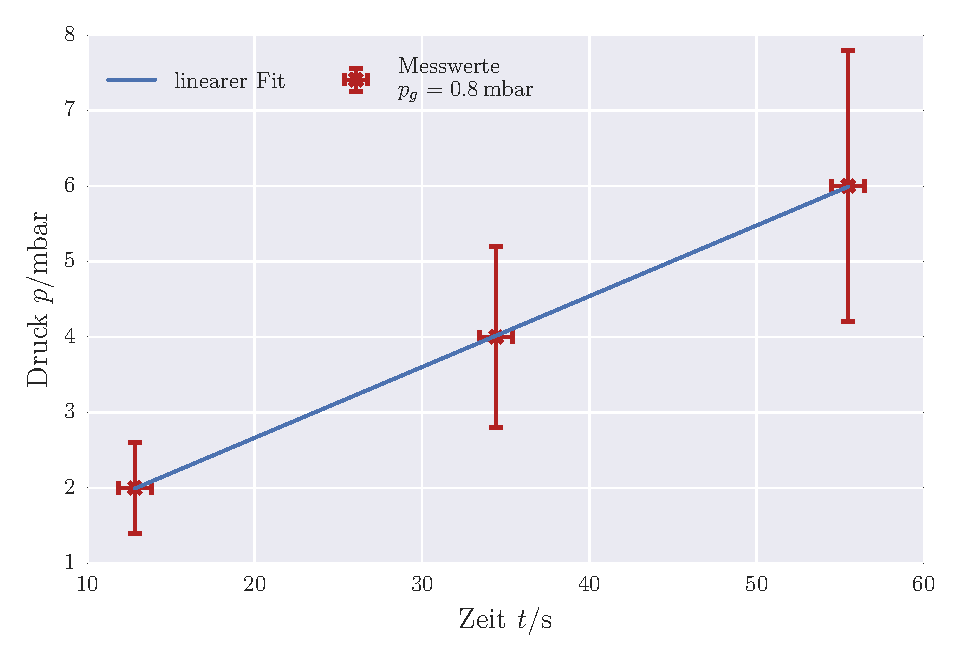
\includegraphics[scale=0.8]{../Grafiken/Leckrate_Drehschieber_3.pdf}
 \caption{Graphische Darstellung der Druckmesswerte in Abhängigkeit von der Zeit, aus der 4. Messreihe, und der
 entsprechenden Ausgleichsgeraden. Der für die Messreihe eingestellte Gleichgewichtsdruck ist angegeben und als Messwert für $t=0$ mit eingetragen. Dieser ist grau dargestellt, da er für die 
 Berechnung der Ausgleichsgeraden nicht verwendet wurde. \label{fig:leckrate_drehschieber_3}}
 \end{figure} 
\FloatBarrier}

Die durchgeführte lineare Ausgleichsrechnung für jede Messreihe ergab, für eine Gerade der Form
\begin{empheq}{equation}
p_{i}(t) = c_{i} \cdot t + d_{i},
\end{empheq}
die jeweiligen Fit-Parameter:


{% Kopierte Ergebnisse
% a =  0.00343320969805 +/- 0.000232609369483
% b =  0.16437881839 +/- 0.0194087844156
%Saugvermögen 0.35+/-0.05

%a =  0.00734136153034 +/- 0.000159807738651
%b =  0.267199767693 +/- 0.00806919876938
%Saugvermögen 0.37+/-0.05

%a =  0.0112064202218 +/- 0.00283513818665
%b =  0.534856097298 +/- 0.0781266429063
%Saugvermögen 0.29+/-0.08

%a =  0.0938182823124 +/- 0.000686074570844
%b =  0.786723830802 +/- 0.0263582331142
%Saugvermögen 1.19+/-0.14
}
\addtocounter{equation}{-1}

{%Mit Minipages 2x2
%\begin{subequations}
%	\begin{minipage}[]{0.5\textwidth}
%		\begin{empheq}{align}
%		c_{1} &=\SI{0.0034(2)}{\milli\bar\per\s}\\ 
%		d_{1} &=\SI{0.16(2)}{} 
%		\end{empheq}	                                                                                  
%		\begin{empheq}{align}
%		c_{2} &=\SI{0.0073(2)}{\milli\bar\per\s}\\ 
%		d_{2} &=\SI{0.267(8)}{} 
%		\end{empheq}
%	\end{minipage}
%	\begin{minipage}[c]{0.5\textwidth}
%		\begin{empheq}{align}
%		c_{3} &=\SI{0.011(3)}{\milli\bar\per\s}\\ 
%		d_{3} &=\SI{0.53(8)}{} 
%		\end{empheq}
%		\begin{empheq}{align}
%		c_{4} &=\SI{0.0938(7)}{\milli\bar\per\s}\\ 
%		d_{4} &=\SI{0.79(3)}{} 
%		\end{empheq}
%	\end{minipage}	
%\end{subequations}\\
}

\begin{subequations}
	\begin{empheq}{align}
	c_{1} &=\SI{0.0034(2)}{\milli\bar\per\s}\\ 
	d_{1} &=\SI{0.16(2)}{} \notag
	\end{empheq}	                                                                                  
	\begin{empheq}{align}
	c_{2} &=\SI{0.0073(2)}{\milli\bar\per\s}\\ 
	d_{2} &=\SI{0.267(8)}{} \notag
	\end{empheq}
	\begin{empheq}{align}
	c_{3} &=\SI{0.011(3)}{\milli\bar\per\s}\\ 
	d_{3} &=\SI{0.53(8)}{} \notag
	\end{empheq}
	\begin{empheq}{align}
	c_{4} &=\SI{0.0938(7)}{\milli\bar\per\s}\\ 
	d_{4} &=\SI{0.79(3)}{} \notag
	\end{empheq}	
\end{subequations}\\

Aus den berechneten Steigungen $c_{i}$ der Ausgleichsgeraden kann mit \eqref{eq:Saugvermoegen_Leckrate}
das Saugvermögen der Drehschieberpumpe bestimmt werden. Das dafür notwendige Volumen wurde aus
den Einzelvolumen der Bauteile zu $V_{\mathrm{Leck,dreh}} = \SI{10.2(7)}{\l}$ bestimmt und 
die jeweiligen Gleichgewichtsdrücke sind in den Grafiken in \cref{tab:Saugvermoegen_Drehschieber}
angegeben. Die Werte für das Saugvermögen ergeben sich damit zu:

\begin{subequations}
	\begin{empheq}{align}
	S_{1} &=\SI{0.35(5)}{\l\per\s}\\ 
	S_{2} &=\SI{0.37(5)}{\l\per\s}\\ 
	S_{3} &=\SI{0.29(8)}{\l\per\s}\\
	S_{3} &=\SI{1.2(1)}{\l\per\s}
	\end{empheq}	
\end{subequations}


\subsubsection{Saugvermögen}

Die in den vorherigen Messungen bestimmten Werte für das Saugvermögen der Drehschieberpumpe
sind zusammen mit dem jeweiligen Druck in \cref{tab:Saugvermoegen_Drehschieber} eingetragen
und in \cref{fig:saugvermögen_drehschieber} grafisch dargestellt.

%Tabelle zum Saugvermögen
\begin{table}[!h]
	\centering
	\begin{tabular}{cccc}
		\toprule
		Druck & Saugvermögen & Druck & Saugvermögen\\
		$p$/\si{mbar} & $S$/\si{ls^{-1}} & $p$/\si{mbar} & $S$/\si{ls^{-1}}\\
\midrule
		\num{0.08(2)} & \num{0.14(2)} & \num{0.6(2)} & \num{0.49(4)}\\
		\num{0.10(3)} & \num{0.3(1)} & \num{0.8(2)} & \num{1.2(4)}\\
		\num{0.20(6)} & \num{0.4(1)} & \num{4(1)} & \num{0.97(6)}\\
		\num{0.4(1)} & \num{0.3(1)} & \num{60(18)} & \num{0.50(5)}\\
		\bottomrule
	\end{tabular}
	\caption{Aus den vorherigen Messergebnissen berechnet Werte für das 
                        Saugvermögen der Drehschieberpumpe in Abhängigkeit des jeweiligen Druckes. \label{tab:Saugvermoegen_Drehschieber}}
\end{table}



%Grafik des Saugvermögens
\begin{figure}[!h]
 \centering
 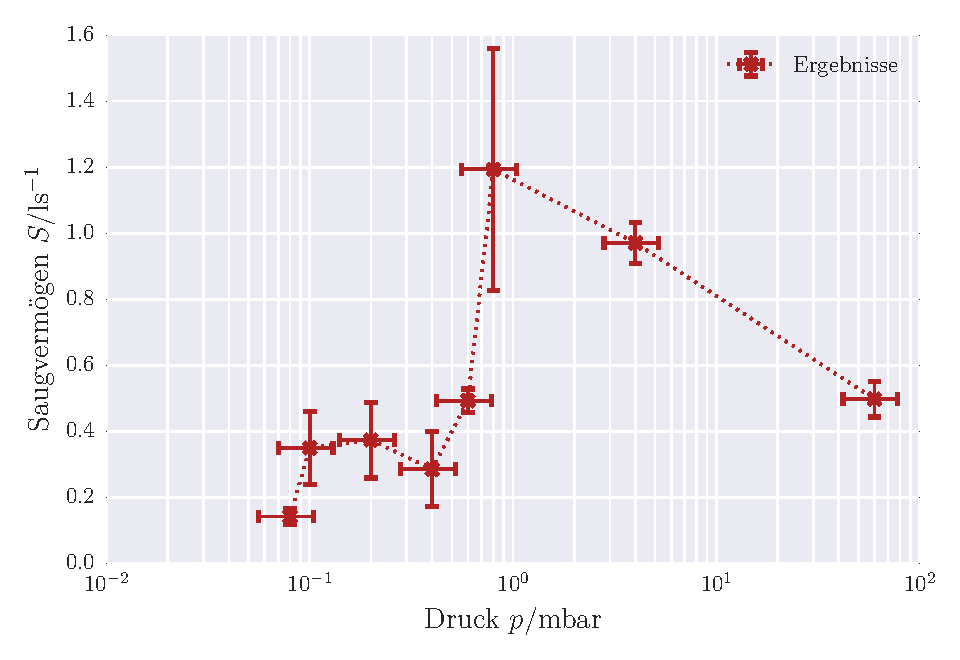
\includegraphics[scale=0.8]{../Grafiken/Saugvermoegen_Drehschieber.pdf}
 \caption{Grafische Darstellung der Ergebnisse für das Saugvermögen aus den vorangegangenen Messreihen in 
 Abhängigkeit des Druckes bei dem sich dieses Saugvermögen ergab. \label{fig:saugvermögen_drehschieber}}
 \end{figure} 
\FloatBarrier

\subsection{Turbopumpe}
In den Folgenden Abschnitten werden die, unter Verwendung der Turbopumpe, aufgenommenen Messreihen 
zur Evakuierungskurve und der Leckratenmessung ausgewertet. Mit den Ergebnissen aus diesen, folgt im letzten Teil dieses 
Abschnitts die Betrachtung des Saugvermögens in Abhängigkeit des Druckes.

\subsubsection{Evakuierungskurve}

%Tabelle der Messwerte
\begin{table}[!h]
	\centering
	\begin{tabular}{cccccc}
		\toprule
		Druck & logarithm. Druck & gemittelte Zeit & Druck & logarithm. Druck & gemittelte Zeit\\
		$p$/\si{10^{-8}\,bar} & $\frac{p-p_e}{p_0-p_e}$ & $\bar{t}$/\si{s} & $p$/\si{10^{-8}\,bar} & $\frac{p-p_e}{p_0-p_e}$ & $\bar{t}$/\si{s}\\
\midrule
		\num{80(8)} & \num{0.0(0)} & \num{5(1)} & \num{9.0(9)} & \num{-2.4(2)} & \num{18(1)}\\
		\num{70(7)} & \num{-0.1(1)} & \num{6(1)} & \num{8.0(8)} & \num{-2.5(2)} & \num{20(1)}\\
		\num{59(6)} & \num{-0.3(1)} & \num{6(1)} & \num{7.0(7)} & \num{-2.7(2)} & \num{22(1)}\\
		\num{50(5)} & \num{-0.5(1)} & \num{7(1)} & \num{6.0(6)} & \num{-2.9(2)} & \num{24(1)}\\
		\num{40(4)} & \num{-0.7(1)} & \num{8(1)} & \num{5.0(5)} & \num{-3.1(2)} & \num{28(1)}\\
		\num{29(3)} & \num{-1.0(1)} & \num{9(1)} & \num{4.0(4)} & \num{-3.5(2)} & \num{34(1)}\\
		\num{20(2)} & \num{-1.4(1)} & \num{12(1)} & \num{3.0(3)} & \num{-4.0(3)} & \num{48(1)}\\
		\num{10(1)} & \num{-2.2(2)} & \num{17(1)}\\
		\bottomrule
	\end{tabular}
	\caption{Werte der Messung der Evakuierungskurve unter Verwendung der Turbopumpe.
                        Neben den gemessenen Drücken sind auch die logarithmierten Drücke und die gemittelten
                        Zeiten angegeben. Dabei sind die Fehler der Zeiten systematischen Ursprungs und wurden 
                        daher durch das Mitteln nicht reduziert. \label{tab:Evakuierungskurve_Turbo}}
\end{table}


{%Exponential-Darstellung der Messdaten
\begin{figure}[!h]
 \centering
 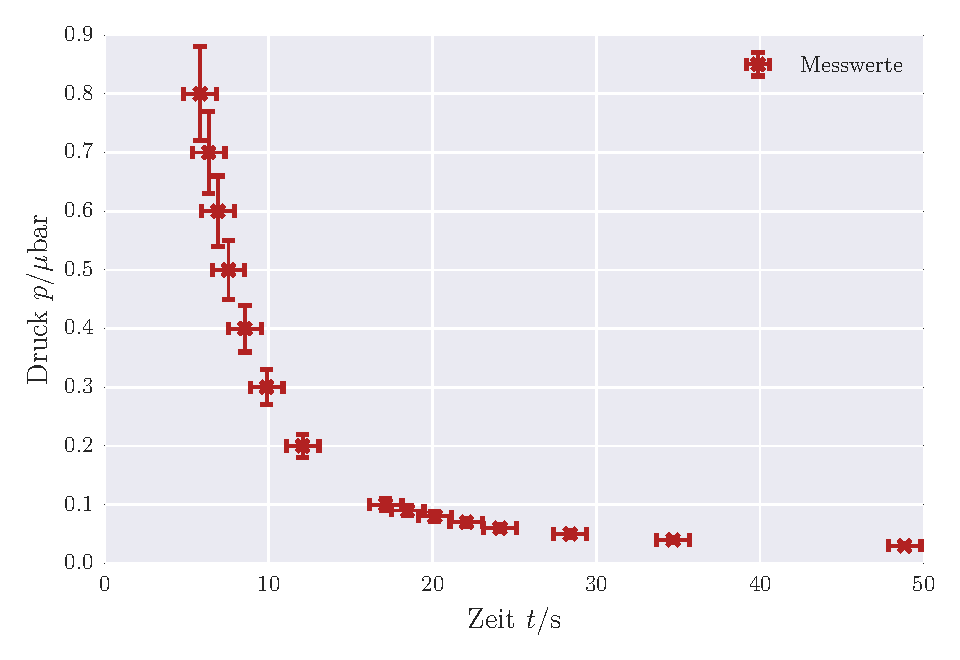
\includegraphics[scale=0.9]{../Grafiken/Evakuierungskurve_Turbo_exp.pdf}
 \caption{Grafische Darstellung der aufgenommenen Evakuierungskurve der Turbopumpe.\label{fig:evakuierungskurve_turbo_exp}}
 \end{figure} 
\FloatBarrier}

{%Logarithmische-Darstellung der Messdaten mit Fits
\begin{figure}[!h]
 \centering
 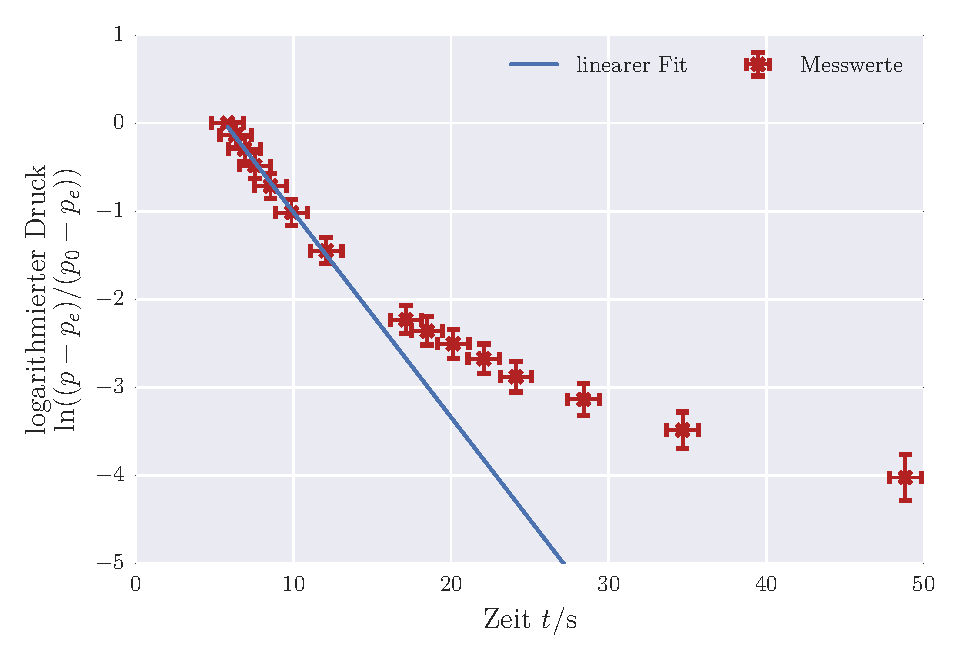
\includegraphics[scale=0.8]{../Grafiken/Evakuierungskurve_Turbo_log_0.pdf}
 \caption{Grafische Darstellung der Evakuierungskurve mit logarithmierten Druckmesswerten und der Ausgleichsgrade für den ersten Druckbereich (\SI{0.8}{\micro\bar} bis \SI{0.6}{\micro\bar})\label{fig:evakuierungskurve_turbo_log_0}}
 \end{figure} 
\FloatBarrier
\begin{figure}[!h]
 \centering
 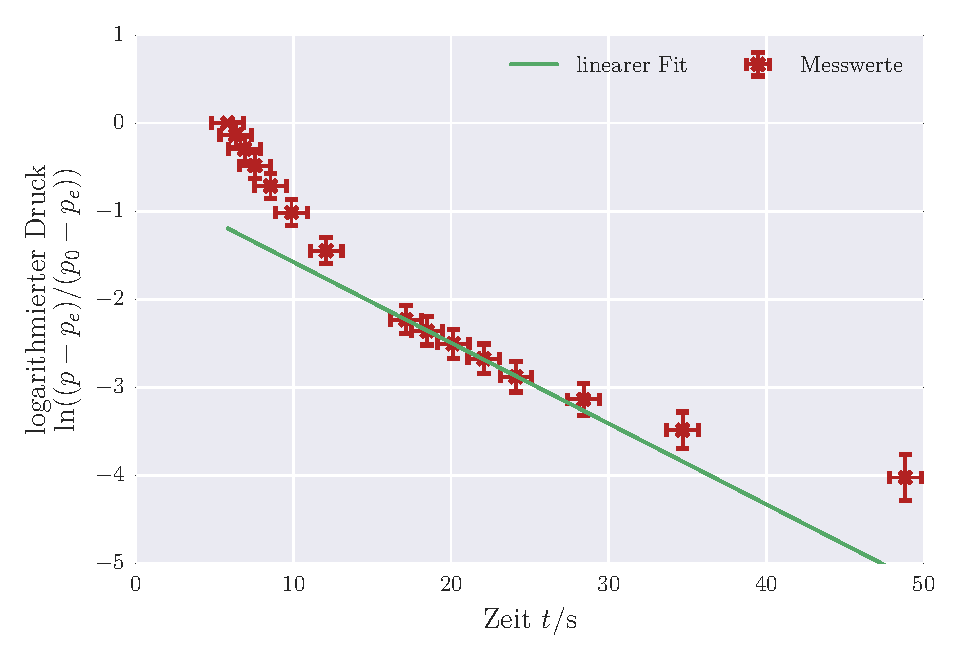
\includegraphics[scale=0.8]{../Grafiken/Evakuierungskurve_Turbo_log_1.pdf}
 \caption{Grafische Darstellung der Evakuierungskurve mit logarithmierten Druckmesswerten und der Ausgleichsgrade für den zweiten Druckbereich (\SI{0.5}{\micro\bar} bis \SI{0.2}{\micro\bar})\label{fig:evakuierungskurve_turbo_log_1}}
 \end{figure} 
\FloatBarrier
\begin{figure}[!h]
 \centering
 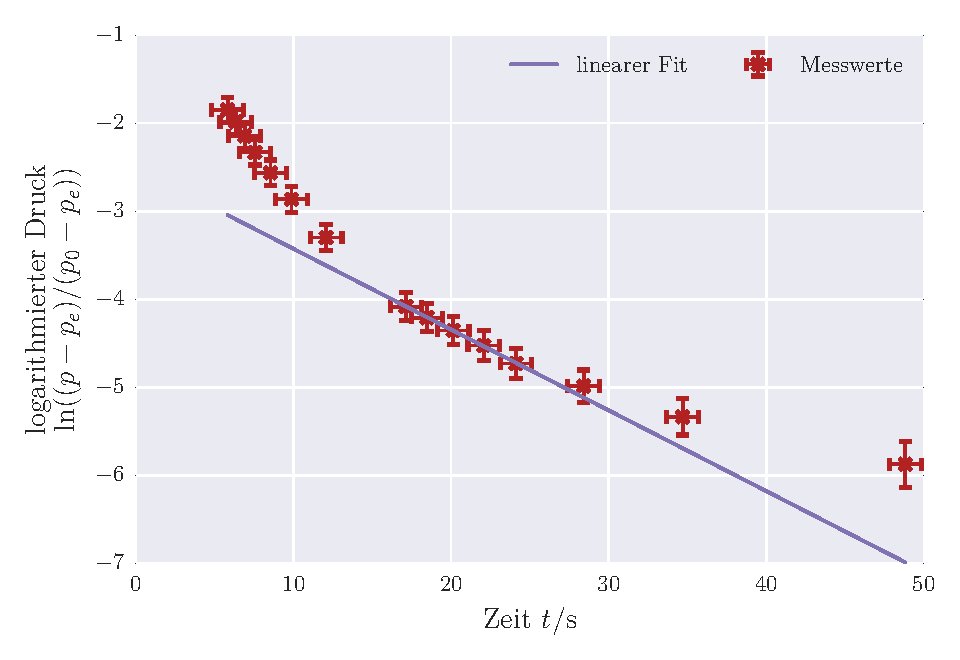
\includegraphics[scale=0.9]{../Grafiken/Evakuierungskurve_Turbo_log_2.pdf}
 \caption{Grafische Darstellung der Evakuierungskurve mit logarithmierten Druckmesswerten und der Ausgleichsgrade für den dritten Druckbereich (\SI{50}{\nano\bar} bis \SI{30}{\nano\bar})\label{fig:evakuierungskurve_turbo_log_2}}
 \end{figure} 
\FloatBarrier}

\subsubsection{Leckratenmessung}
% Tabelle der Lecktratenmessung
\begin{table}[!h]
	\centering
	\subfloat{
	\begin{tabular}{cccc}
		\toprule
		\multicolumn{2}{c}{1.Messreihe $P_g = \SI{4.0(4)e-08}{\bar}$} & \multicolumn{2}{c}{2.Messreihe $P_g = \SI{6.0(6)e-08}{\bar}$} \\\cmidrule(rl){1-2}\cmidrule(rl){3-4}
		Druck & gemittelte Zeit & Druck & gemittelte Zeit\\
		$p$/\si{10^{-8}bar} & $\bar{t}$/\si{s} & $p$/\si{10^{-8}bar} & $\bar{t}$/\si{s}\\
		\midrule
		\num{20(2)} & \num{5(1)} & \num{20(2)} & \num{1(1)}\\
		\num{30(3)} & \num{8(1)} & \num{30(3)} & \num{2(1)}\\
		\num{40(4)} & \num{11(1)} & \num{40(4)} & \num{4(1)}\\
					&			& \num{50(5)} & \num{6(1)}\\
		\bottomrule
%	\end{tabular}
%	}\\
%	\subfloat{
%	\begin{tabular}{cccc}
		\toprule
		\multicolumn{2}{c}{3.Messreihe $P_g = \SI{8.0(8)e-08}{\bar}$} & \multicolumn{2}{c}{4.Messreihe $P_g = \SI{1.0(1)e-07}{\bar}$} \\\cmidrule(rl){1-2}\cmidrule(rl){3-4}
		Druck & gemittelte Zeit & Druck & gemittelte Zeit\\
		$p$/\si{10^{-8}bar} & $\bar{t}$/\si{s} & $p$/\si{10^{-8}bar} & $\bar{t}$/\si{s}\\
		\midrule
		\num{30(9)} & \num{1(1)} & \num{40(12)} & \num{2(1)}\\
		\num{40(12)} & \num{2(1)} & \num{50(15)} & \num{2(1)}\\
		\num{50(15)} & \num{3(1)} & \num{60(18)} & \num{3(1)}\\
		\num{60(18)} & \num{6(1)} & \num{70(21)} & \num{4(1)}\\
		\bottomrule
	\end{tabular}
	}
	
	\caption{Werte der Leckratenmessung unter Verwendung der Turbopumpe.
		Neben den gemessenen Drücken sind die gemittelten Zeiten angegeben. 
		Dabei sind die Fehler der Zeiten systematischen Ursprungs und wurden 
		daher durch das Mitteln nicht reduziert. \label{tab:Leckratenmessung_Turbo}}
\end{table}


{%Grafiken der Leckratenmessung
\begin{figure}[!h]
 \centering 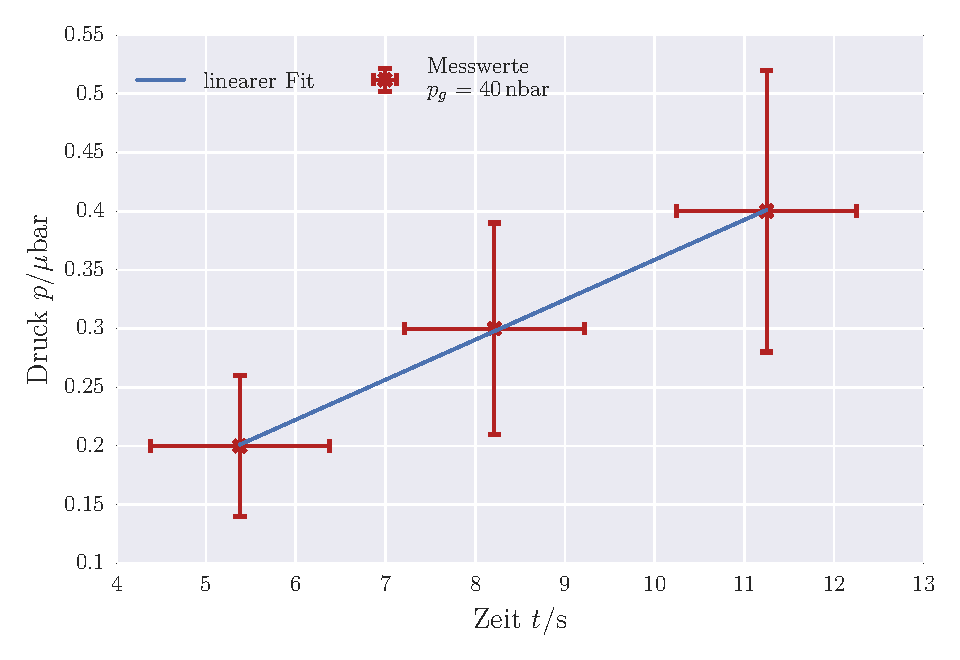
\includegraphics[scale=0.8]{../Grafiken/Leckrate_Turbo_0.pdf}                                                          
 \caption{Graphische Darstellung der Druckmesswerte in Abhängigkeit von der Zeit, aus der 1. Messreihe, und der
 	entsprechenden Ausgleichsgeraden. Der für die Messreihe eingestellte Gleichgewichtsdruck ist angegeben. \label{fig:leckrate_turbo_0}}
 \end{figure} 
\FloatBarrier

\begin{figure}[!h]
 \centering
 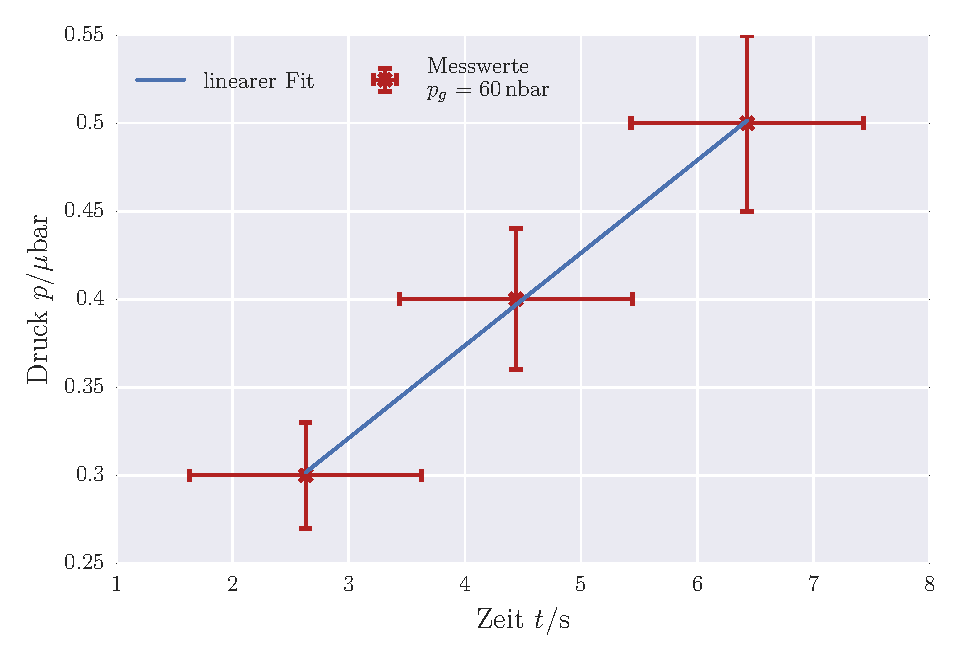
\includegraphics[scale=0.65]{../Grafiken/Leckrate_Turbo_1.pdf}	
 \caption{Graphische Darstellung der Druckmesswerte in Abhängigkeit von der Zeit, aus der 2. Messreihe, und der
 	entsprechenden Ausgleichsgeraden. Der für die Messreihe eingestellte Gleichgewichtsdruck ist angegeben und als Messwert für $t=0$ mit eingetragen. Dieser ist grau dargestellt, da er für die 
 	Berechnung der Ausgleichsgeraden nicht verwendet wurde. Diese Auslassung wurde vorgenommen, da
 	der tatsächliche Druck bei $t=0$, durch den plötzlichen Druckanstieg bei Schließung des Ventils zur Pumpe, von dem
 	gemessenen Druck bei offenem Ventil abweicht.
 \label{fig:leckrate_turbo_1}}
 \end{figure} 
\FloatBarrier
\begin{figure}[!h]
 \centering
 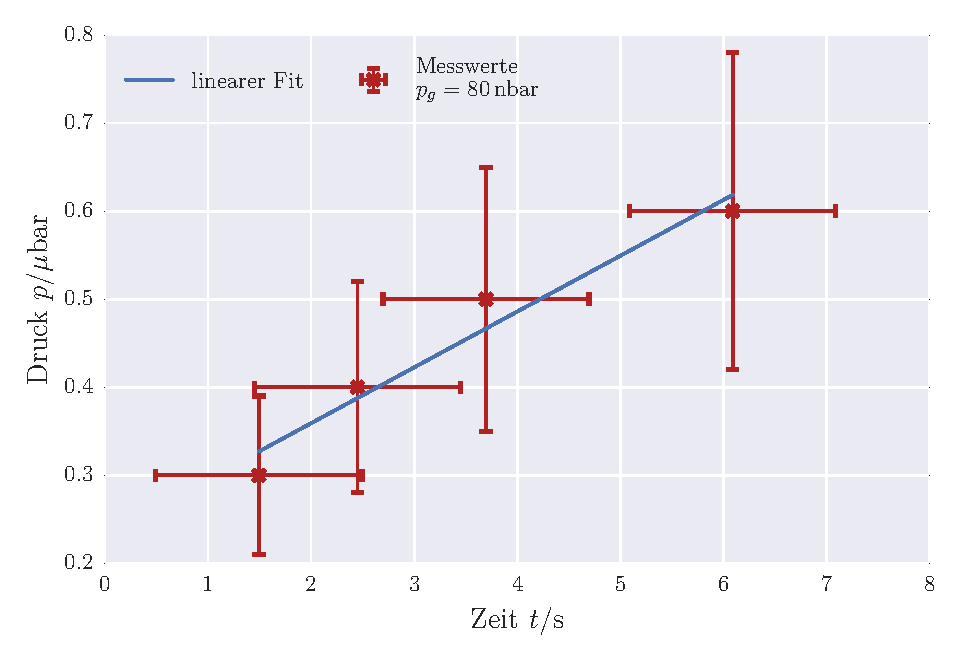
\includegraphics[scale=0.65]{../Grafiken/Leckrate_Turbo_2.pdf}
 \caption{Graphische Darstellung der Druckmesswerte in Abhängigkeit von der Zeit, aus der 3. Messreihe, und der
 	entsprechenden Ausgleichsgeraden. Der für die Messreihe eingestellte Gleichgewichtsdruck ist angegeben und als Messwert für $t=0$ mit eingetragen. Dieser ist grau dargestellt, da er für die 
 	Berechnung der Ausgleichsgeraden nicht verwendet wurde. Diese Auslassung wurde vorgenommen, da
 	der tatsächliche Druck bei $t=0$, durch den plötzlichen Druckanstieg bei Schließung des Ventils zur Pumpe, von dem
 	gemessenen Druck bei offenem Ventil abweicht.  \label{fig:leckrate_turbo_2}}
 \end{figure} 
\FloatBarrier
\begin{figure}[!h]
 \centering
 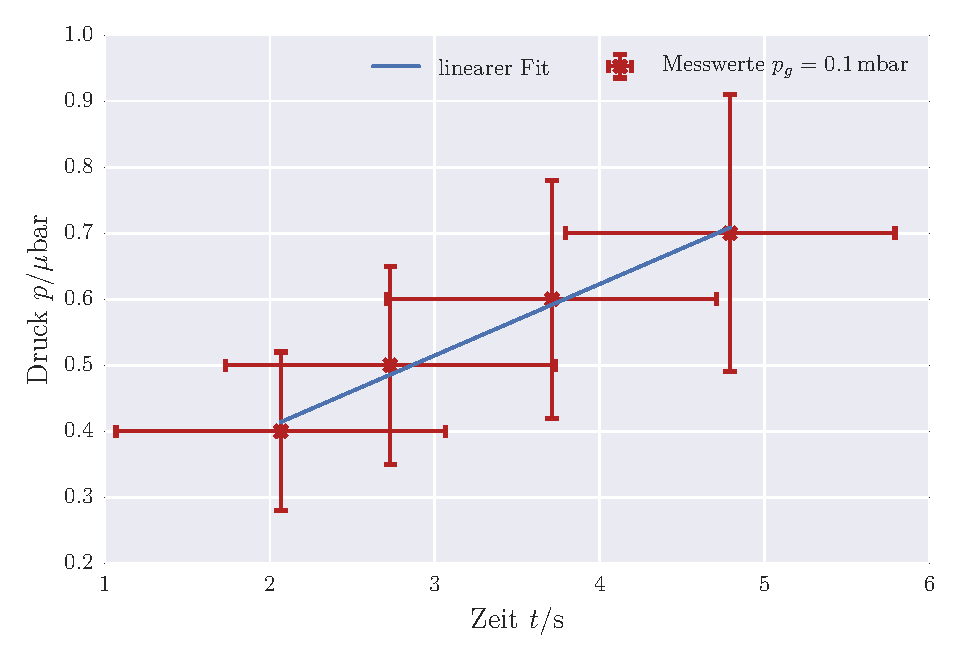
\includegraphics[scale=0.65]{../Grafiken/Leckrate_Turbo_3.pdf}
 \caption{Graphische Darstellung der Druckmesswerte in Abhängigkeit von der Zeit, aus der 4. Messreihe, und der
 	entsprechenden Ausgleichsgeraden. Der für die Messreihe eingestellte Gleichgewichtsdruck ist angegeben und als Messwert für $t=0$ mit eingetragen. Dieser ist grau dargestellt, da er für die 
 	Berechnung der Ausgleichsgeraden nicht verwendet wurde. Diese Auslassung wurde vorgenommen, da
 	der tatsächliche Druck bei $t=0$, durch den plötzlichen Druckanstieg bei Schließung des Ventils zur Pumpe, von dem
 	gemessenen Druck bei offenem Ventil abweicht.  \label{fig:leckrate_turbo_3}}
 \end{figure} 
\FloatBarrier}

\subsubsection{Saugvermögen}
%Tabelle zum Saugvermögen
\begin{table}[!h]
	\centering
	\begin{tabular}{cccc}
		\toprule
		Druck & Saugvermögen & Druck & Saugvermögen\\
		$p$/\si{10^{-8}\,bar} & $S$/\si{ls^{-1}} & $p$/\si{10^{-8}\,bar} & $S$/\si{ls^{-1}}\\
\midrule
		\num{4.0(4)} & \num{8(1)} & \num{9.0(9)} & \num{0.92(6)}\\
		\num{5.0(5)} & \num{0.43(5)} & \num{10(1)} & \num{10(2)}\\
		\num{6.0(6)} & \num{8(1)} & \num{40(4)} & \num{2.1(2)}\\
		\num{8.0(8)} & \num{8(2)} & \num{70(7)} & \num{2.7(2)}\\
		\bottomrule
	\end{tabular}
	\caption{Aus den vorherigen Messergebnissen berechnet Werte für das 
                       Saugvermögen der Turbopumpe in Abhängigkeit des jeweiligen Druckes. \label{tab:Saugvermoegen_Drehschieber}}
\end{table}


%Grafik des Saugvermögens
\begin{figure}[!h]
 \centering
 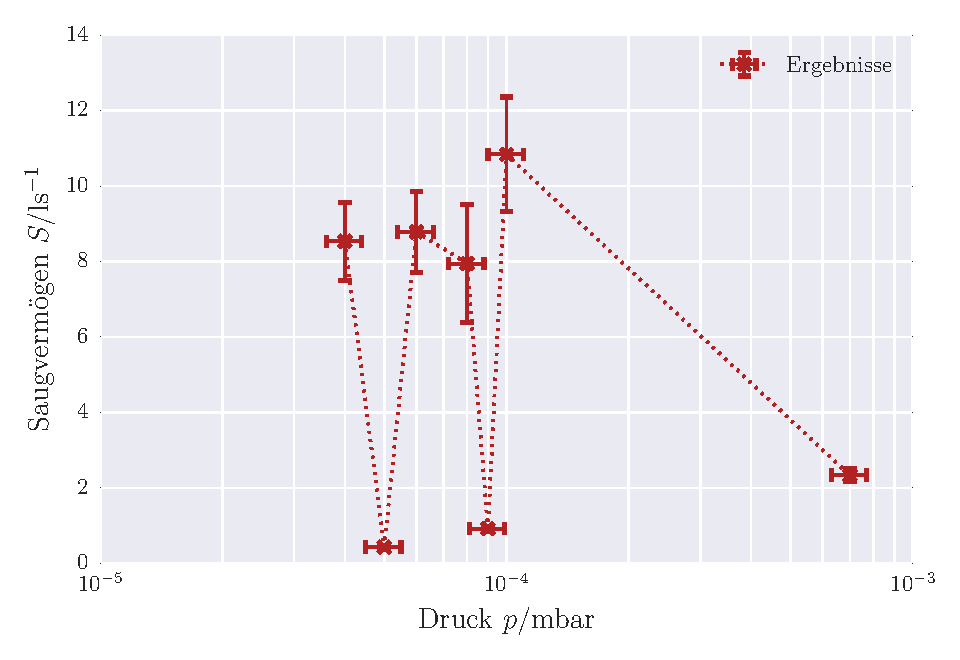
\includegraphics[scale=0.9]{../Grafiken/Saugvermoegen_Turbo.pdf}
 \caption{Grafische Darstellung der Ergebnisse für das Saugvermögen aus den vorangegangenen Messreihen in 
 	Abhängigkeit des Druckes bei dem sich dieses Saugvermögen ergab. \label{fig:saugvermögen_turbo}}
 \end{figure} 
\FloatBarrier









